% Options for packages loaded elsewhere
\PassOptionsToPackage{unicode}{hyperref}
\PassOptionsToPackage{hyphens}{url}
%
\documentclass[
]{book}
\usepackage{amsmath,amssymb}
\usepackage{lmodern}
\usepackage{iftex}
\ifPDFTeX
  \usepackage[T1]{fontenc}
  \usepackage[utf8]{inputenc}
  \usepackage{textcomp} % provide euro and other symbols
\else % if luatex or xetex
  \usepackage{unicode-math}
  \defaultfontfeatures{Scale=MatchLowercase}
  \defaultfontfeatures[\rmfamily]{Ligatures=TeX,Scale=1}
\fi
% Use upquote if available, for straight quotes in verbatim environments
\IfFileExists{upquote.sty}{\usepackage{upquote}}{}
\IfFileExists{microtype.sty}{% use microtype if available
  \usepackage[]{microtype}
  \UseMicrotypeSet[protrusion]{basicmath} % disable protrusion for tt fonts
}{}
\makeatletter
\@ifundefined{KOMAClassName}{% if non-KOMA class
  \IfFileExists{parskip.sty}{%
    \usepackage{parskip}
  }{% else
    \setlength{\parindent}{0pt}
    \setlength{\parskip}{6pt plus 2pt minus 1pt}}
}{% if KOMA class
  \KOMAoptions{parskip=half}}
\makeatother
\usepackage{xcolor}
\IfFileExists{xurl.sty}{\usepackage{xurl}}{} % add URL line breaks if available
\IfFileExists{bookmark.sty}{\usepackage{bookmark}}{\usepackage{hyperref}}
\hypersetup{
  pdftitle={Power BI Primer},
  hidelinks,
  pdfcreator={LaTeX via pandoc}}
\urlstyle{same} % disable monospaced font for URLs
\usepackage{longtable,booktabs,array}
\usepackage{calc} % for calculating minipage widths
% Correct order of tables after \paragraph or \subparagraph
\usepackage{etoolbox}
\makeatletter
\patchcmd\longtable{\par}{\if@noskipsec\mbox{}\fi\par}{}{}
\makeatother
% Allow footnotes in longtable head/foot
\IfFileExists{footnotehyper.sty}{\usepackage{footnotehyper}}{\usepackage{footnote}}
\makesavenoteenv{longtable}
\usepackage{graphicx}
\makeatletter
\def\maxwidth{\ifdim\Gin@nat@width>\linewidth\linewidth\else\Gin@nat@width\fi}
\def\maxheight{\ifdim\Gin@nat@height>\textheight\textheight\else\Gin@nat@height\fi}
\makeatother
% Scale images if necessary, so that they will not overflow the page
% margins by default, and it is still possible to overwrite the defaults
% using explicit options in \includegraphics[width, height, ...]{}
\setkeys{Gin}{width=\maxwidth,height=\maxheight,keepaspectratio}
% Set default figure placement to htbp
\makeatletter
\def\fps@figure{htbp}
\makeatother
\setlength{\emergencystretch}{3em} % prevent overfull lines
\providecommand{\tightlist}{%
  \setlength{\itemsep}{0pt}\setlength{\parskip}{0pt}}
\setcounter{secnumdepth}{5}
\usepackage{booktabs}
\ifLuaTeX
  \usepackage{selnolig}  % disable illegal ligatures
\fi
\usepackage[]{natbib}
\bibliographystyle{apalike}

\title{Power BI Primer}
\author{}
\date{\vspace{-2.5em}2022-08-13}

\begin{document}
\maketitle

{
\setcounter{tocdepth}{1}
\tableofcontents
}
\hypertarget{Power-BI-Primer}{%
\chapter*{Power BI Primer}\label{Power-BI-Primer}}
\addcontentsline{toc}{chapter}{Power BI Primer}

\begin{center}\rule{0.5\linewidth}{0.5pt}\end{center}

\textbf{What is this?}

This book is designed to provide readers with a brief introduction to Power BI. It is not intended to provide a comprehensive overview of all the features of Power BI, it should however provider users with enough information to start transforming and visualising data either to produce an interactive visualisation or a dashboard.

\textbf{Contents}

\begin{itemize}
\tightlist
\item
  Power BI

  \begin{itemize}
  \tightlist
  \item
    Introduction
  \item
    Getting Started
  \item
    Data Transformation Basics
  \item
    Data Visualisation
  \item
    Adding New Pages
  \item
    Navigation
  \item
    Indexing
  \item
    Relationships
  \item
    Publishing
  \item
    Sharing
  \item
    Additional Resources
  \end{itemize}
\end{itemize}

\hypertarget{intro}{%
\chapter{Introduction}\label{intro}}

\begin{center}\rule{0.5\linewidth}{0.5pt}\end{center}

\hypertarget{introduction}{%
\section{Introduction}\label{introduction}}

\textbf{Power BI} is part of the \textbf{Microsoft Power Platform} which includes other packages such as Power Automate. Power BI is split into several components: Power BI Desktop, Service (an online SaaS - Software as a Service), Gateway, Report Server, Premium, Visuals Marketplace and Mobile Apps. The primary focus of Power BI is business intelligence but Power BI can be used for more than standard reporting of data with line charts and bar charts. It can also be used in conjunction with Python and R to create complex custom visuals or it can be used to create and train \href{https://docs.microsoft.com/en-us/power-bi/connect-data/service-tutorial-build-machine-learning-model}{machine learning models}. Power BI can even be used to \href{https://docs.microsoft.com/en-us/power-bi/connect-data/desktop-connect-to-web-by-example}{web scrape data}.

With Power BI Desktop, you can connect to different data sources, transform those data sources through queries, build data models and create visualizations and reports or dashboards for different audiences. Reports and dashboards can be published to the Power BI Service where you can share your reports with other users or a wider audience.

This document is intended to provide a broad overview of the features of Power BI Desktop reports to provide the reader with the necessary tools to start learning and exploring Power BI for themselves. It covers the basics such as importing data, transforming data, visualizing data, using slicer visuals, navigation and basic UI design.

\hypertarget{getting-started}{%
\chapter{Getting Started}\label{getting-started}}

\begin{center}\rule{0.5\linewidth}{0.5pt}\end{center}

\hypertarget{downloading-and-installing-power-bi}{%
\section{Downloading and Installing Power BI}\label{downloading-and-installing-power-bi}}

To download Power BI Desktop, go to the Power BI Desktop download page and select \textbf{Download Free}. You can also download Power BI Desktop from the Power BI service. Select the \textbf{Download} icon in the top menu bar, and then select Power BI Desktop.

\hypertarget{launching-power-bi}{%
\section{Launching Power BI}\label{launching-power-bi}}

Once you launch Power BI Desktop you will be welcomed by the \textbf{Start screen}. Here, you can get data sources for your reports, watch video tutorials, check updates and visit the Power BI forums. For now, select the \textbf{close} icon to close the Welcome screen to see the main interface (Figure 1 below).

\begin{figure}
\centering
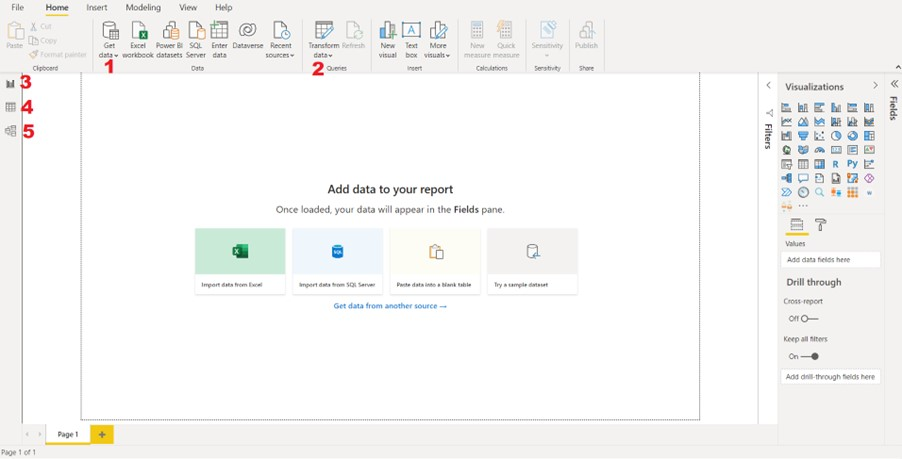
\includegraphics{bi1.jpg}
\caption{Screenshot of the Power BI User Interface.}
\end{figure}

\hypertarget{important-features}{%
\section{Important Features}\label{important-features}}

The image above shows some of the most important features in Power BI Desktop.

\begin{enumerate}
\def\labelenumi{\arabic{enumi}.}
\item
  \textbf{Get data}: This is used for selecting, connecting to and configuring the data sources that will be used in a report or dashboard. A single data source can be used or multiple can be used. When a data source is selected Power BI will provide you with an option to either load the data or transform it. It's worth noting that data source will be stored in Power BI's internal memory, so the more data sources you connect to and the larger those sources are the slower your report/dashboard will run.
\item
  \textbf{Transform data}: This is used to launch the Power Query Editor. The Power Query Editor is where data can be transformed. Transformation usually refers to dealing with missing values or cleaning the data before analysis. The Power Query Editor is a useful tool when working with data sets which need to be cleaned. Working with Power Query Editor is similar to working with Excel and often it is useful to switch between the two as some transformations will be easier in one than the other.
\item
  \textbf{Report View or canvas}: The report view icon opens the report view canvas which is used for selecting and designing data visualizations. This is the default view open when Power BI is launched.
\item
  \textbf{Data View}: The data view allows you to view all the data available in your report. This view looks similar to an Excel spreadsheet but it is read only. It is useful to quickly check data types, validate data and make small changes to your data source - such as changing a data type or the format of a variable.
\item
  \textbf{Model View or Relationship View}: The relationship or model view allows you to set relationships between data sources. Relationships occur where two or more data sources are linked together by related data (a shared variable like `year' for instance).
\end{enumerate}

\hypertarget{loading-data-excel}{%
\section{Loading Data (Excel)}\label{loading-data-excel}}

We're going to use a dummy dataset health\_data.xlsx included in the \href{https://github.com/aamcmurray/BookTest/blob/main/health_data.xlsx}{repository used to host this guide}. Download and save the dataset in a folder you can easily locate.

To use Excel data sets as a source, open the Power BI Desktop. Under the \textbf{Home ribbon} find \textbf{Get Data}. Selecting the down arrow next to the Get Data button will show the most common connectors used but clicking the button itself will provide a full list of all available connectors. The list is extensive and Power BI can connect to a wide array of data sources including .csv files, .xlsx and .txt files. Power BI also supports SQL database connections. Whether you click the Get Data button or the arrow you will see Excel at the top of the resulting list. Click \textbf{Excel Workbook} and then click Connect. Navigate to your data source.

Once selected you will see two separate spreadsheets you can choose from.

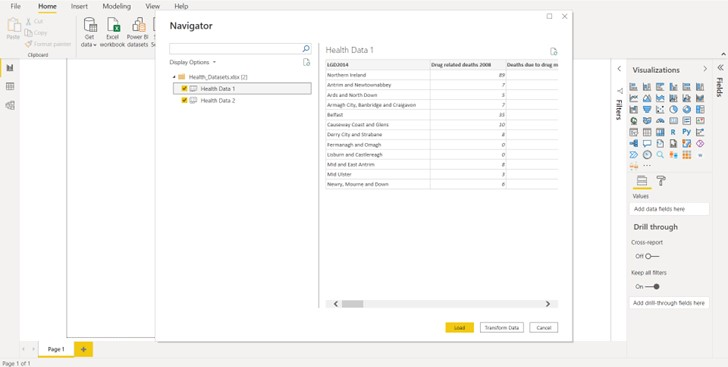
\includegraphics{bi2.jpg}
Clicking once on the spreadsheet name will let you preview the data while clicking on the \textbf{checkbox} next to the name will include it as part of the data import. Here we have two sheets, Health Data 1 which contains data relating to drug related deaths and deaths due to drug misuse and Health Data 2 which contains population data. This data needs to be cleaned before we can use it so tick both the boxes and then press the \textbf{Transform Data} button on the bottom of the panel. This launches the \textbf{Power Query Editor}. You can also clean your data in Excel then simply press the Load button but some data sets would be too difficult to transform in Excel.

\hypertarget{power-query-editor}{%
\section{Power Query Editor}\label{power-query-editor}}

When the Power Query Editor loads you will notice it has its own environment.

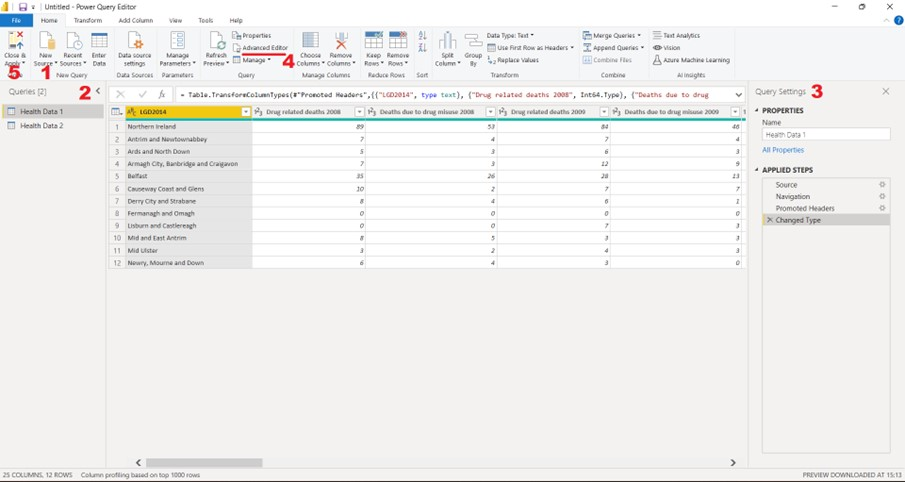
\includegraphics{bi3.jpg}
There are a number of features in the Power Query Editor to take note of:

\begin{enumerate}
\def\labelenumi{\arabic{enumi}.}
\item
  \textbf{New Source}: This launches the same interface as the Get Data button.
\item
  \textbf{Queries Pane}: The queries pane is a list of all the queries that you have connected to.
\item
  \textbf{Query Settings}: Within this pane you can see the complete history of transformations that have been applied to your query. You can also rename the query. This history is useful for several reasons. From here you can rename a query, or click the `x' beside a query to remove a query, and reorder queries by clicking and dragging them into different positions.
\item
  \textbf{Advanced Editor}: Power Query Editor uses a programming language informally known as M in the background and when you click any button in the Power Query GUI some M code is generated in the background corresponding to what has been done. By launching the Advanced Editory you can see the M query that is automatically written for you by the Power Query Editor.
\item
  \textbf{Close and Apply}: Choosing this option will save your transformations, close the Power Query Editor and load the transformed data into the data model.
\end{enumerate}

The Power Query Editor allows you to transform the data with step-by-step instructions for adjusting the data. Transforming the data this way \textbf{does not affect the original data source}, only this particular view of the data. Data transformation includes a range of processes including: renaming columns or tables, removing rows, replacing missing data entries or changing data types. Power Query Editor records the steps taken to transform the data sequentially under \textbf{Applied Steps} in the \textbf{Query Settings} pane. If you make a mistake or transform the data in a way you aren't happy with you can simply cancel the transformation by clicking the \textbf{X} that appears beside it in \textbf{Applied Steps}.

\hypertarget{data-transformation-basics}{%
\chapter{Data Transformation Basics}\label{data-transformation-basics}}

\begin{center}\rule{0.5\linewidth}{0.5pt}\end{center}

\hypertarget{data-transformation-basics-1}{%
\section{Data Transformation Basics}\label{data-transformation-basics-1}}

In its current format the data contained in Health Data 1 will be hard to visualize in Power BI. We essentially have two data sets in one. The quantitative data is tied up with qualitative data (Drug related deaths 2008). Ideally, we would like the data to look like this:

\begin{longtable}[]{@{}
  >{\raggedleft\arraybackslash}p{(\columnwidth - 6\tabcolsep) * \real{0.3256}}
  >{\raggedleft\arraybackslash}p{(\columnwidth - 6\tabcolsep) * \real{0.2558}}
  >{\raggedleft\arraybackslash}p{(\columnwidth - 6\tabcolsep) * \real{0.2093}}
  >{\raggedleft\arraybackslash}p{(\columnwidth - 6\tabcolsep) * \real{0.2093}}@{}}
\caption{\label{tab:table1}}\tabularnewline
\toprule
\begin{minipage}[b]{\linewidth}\raggedleft
Location
\end{minipage} & \begin{minipage}[b]{\linewidth}\raggedleft
Dataset
\end{minipage} & \begin{minipage}[b]{\linewidth}\raggedleft
Year
\end{minipage} & \begin{minipage}[b]{\linewidth}\raggedleft
Total
\end{minipage} \\
\midrule
\endfirsthead
\toprule
\begin{minipage}[b]{\linewidth}\raggedleft
Location
\end{minipage} & \begin{minipage}[b]{\linewidth}\raggedleft
Dataset
\end{minipage} & \begin{minipage}[b]{\linewidth}\raggedleft
Year
\end{minipage} & \begin{minipage}[b]{\linewidth}\raggedleft
Total
\end{minipage} \\
\midrule
\endhead
Northern Ireland & Drug related deaths & 2008 & 89 \\
Northern Ireland & Deaths due to drug misuse & 2008 & 53 \\
\ldots{} & \ldots{} & \ldots{} & \ldots{} \\
\bottomrule
\end{longtable}

Note how the \textbf{`year'} data and \textbf{`total'} data now have their own columns.

Power Query Editor can help us get there. If we were to \href{https://support.microsoft.com/en-us/office/unpivot-columns-power-query-0f7bad4b-9ea1-49c1-9d95-f588221c7098}{unpivot} the columns and separate the year into its own column we would arrive at a data set that looks like the table above.

The first step then is to click on the column titled \textbf{``Drug related deaths 2008''} then scroll to the right and \textbf{shift click} on the final column. This will select all but the first column. Right click on any of the selected columns and select \textbf{Unpivot Columns} from the menu. This separates the columns into attribute-value pairs. Next we need to separate out the year data. \textbf{Right click} on the newly generated \textbf{Attribute column} and select \textbf{Split Column} then select \textbf{By Delimiter}.

\begin{figure}
\centering
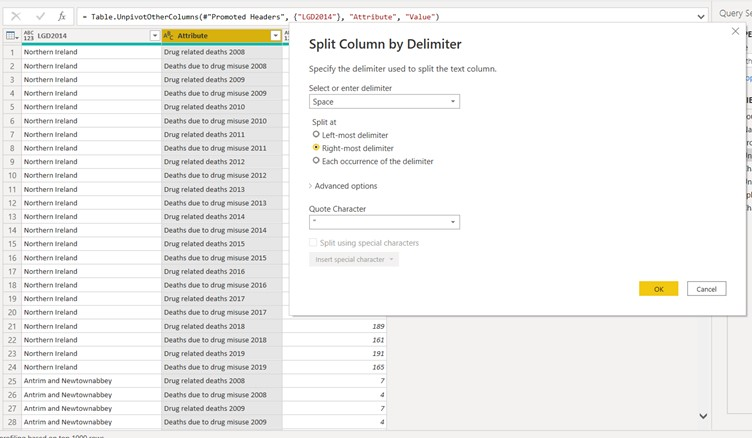
\includegraphics{bi4.jpg}
\caption{Splitting by Delimiters.}
\end{figure}

We want to split this column into two new columns using a delimiter. The best one to choose here is the Space delimiter. We want to split at the \textbf{right-most} delimiter as there is a space right before each year but none after the year. Select these settings and click OK. Change the titles of the columns by \textbf{double clicking} the \textbf{column header}. Finalize your changes by clicking on the \textbf{Home ribbon} and \textbf{Close \& Apply}. As soon as you click Close \& Apply in the Power Query Editor the Power Query Editor will close and the Power BI Desktop Report View will be visible.

These are two of the most common data transformations that data sets will need to have applied to them.

\hypertarget{data-visualisation}{%
\chapter{Data Visualisation}\label{data-visualisation}}

\begin{center}\rule{0.5\linewidth}{0.5pt}\end{center}

\hypertarget{visualising-data}{%
\section{Visualising Data}\label{visualising-data}}

Power BI is commonly associated with the ability to create impactful, interactive data visualizations. Before we start making visuals it's worth detailing some of the panes and views available to us:

\begin{figure}
\centering
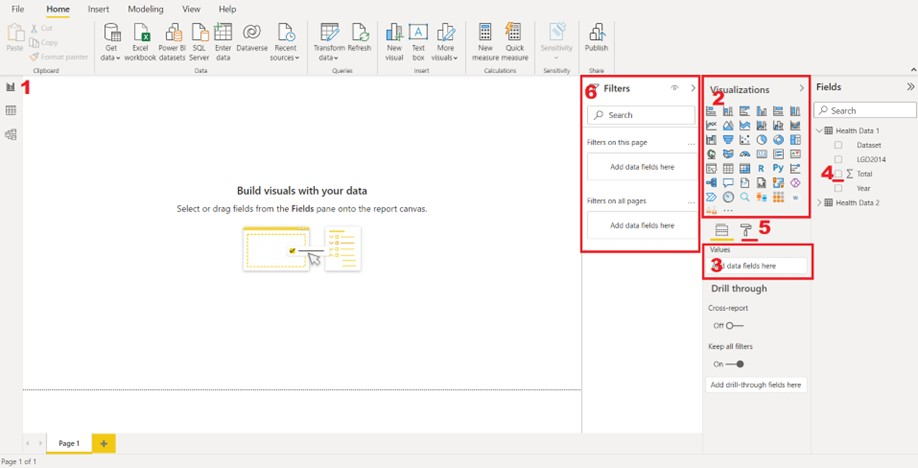
\includegraphics{bi5.jpg}
\caption{Navigating the user interface.}
\end{figure}

\begin{enumerate}
\def\labelenumi{\arabic{enumi}.}
\item
  \textbf{The Report View}: This is the button that will open up the Report canvas and allow us to create visuals using the visuals area. Below the report view button are two more buttons. These provide access to the \textbf{data view} and the \textbf{model view}.
\item
  \textbf{Visuals Area}: This is where we can choose which visual we would like to use. Each of the icons represents a type of visualization. Clicking these icons will generate a visual that we can start to work with. Once custom visuals are added they will appear here as well.
\item
  \textbf{Field Area}: This area will change depending on the visual but it is where we place the variables (Total, Year\ldots{} etc.) that we will use within the selected visual.
\item
  \textbf{Field Pane}: This pane contains the fields we have to choose from to add to our visual. Initially this is populated by the variables contained in data sources but it is possible to add new variables or measures through the Power Query Editor.
\item
  \textbf{Format Area}: This is where we can decide on the formatting of our visuals. You can customise colours or make changes to axes add borders and change font sizes\ldots{} etc.
\item
  \textbf{Filters Area}: This is where we can apply filters of various scopes. We can apply page-level filters which will affect all the visuals on the selected page. We can apply Report-level filters which will affect every visual in the entire Power BI Report and we can apply Visual-level filters which will be applied only to specific visualizations.
\end{enumerate}

\hypertarget{creating-a-line-chart}{%
\subsection{Creating a Line-Chart}\label{creating-a-line-chart}}

We're going to create a \textbf{line-chart visual} that shows both drug related deaths and deaths due to drug misuse. We want to show the totals for each over time and we want to be able to filter by local government district.

The first step in creating any visual is to go to the \textbf{Visualizations pane} on the right-hand side of the UI. Here you can see a range of different visualization icons representing their respective chart. Along the top row are bar charts, in the second row are line charts, area charts and a ribbon chart, below these are pie charts, maps, cards, and even tools to create custom Python and R visuals (Plotly, Matplotlib and Seaborn are three commonly used Python plotting libraries). Find the Icon for the \textbf{Line Chart} and click it. A new visual object will appear on the canvas with a prompt to select or drag fields to populate this visual.

Drag the \textbf{``Year'' field} from the \textbf{fields pane} into the \textbf{Axis box} in the field area. Drag the \textbf{``Total'' field} into the \textbf{Values box}.

You should get a line-chart that looks like this:

\begin{figure}
\centering
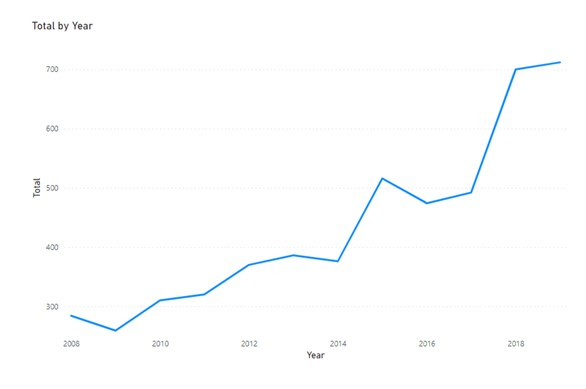
\includegraphics{bi6.jpg}
\caption{The first line chart.}
\end{figure}

There is something not quite right about this visual. We plotted Total by Year but what is it a total of? Our data contained totals for each Local Government District and for two different data sets. Currently, the data for each year is being summed. We are looking at a line chart showing the sum of all Local Government District drug related deaths and deaths due to drug misuse. We can tell this is the case at a glance by looking to the \textbf{Fields Pane} where the \textbf{Total} has a summation sign (\(\sum\)) to the left of it.

Drag the \textbf{Dataset field} into the \textbf{Legend box} to separate out the data sets. You should see a line-chart like this:

\begin{figure}
\centering
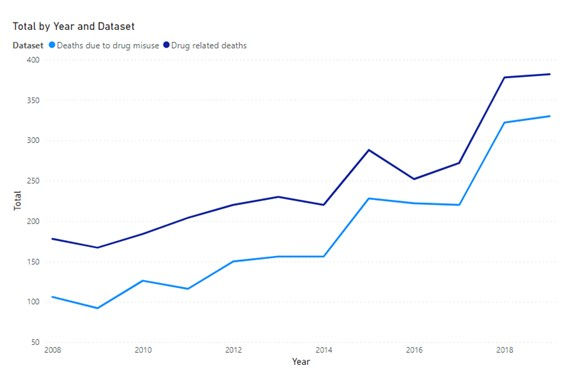
\includegraphics{bi7.jpg}
\caption{Line chart.}
\end{figure}

This is closer to what we had hoped to show but it's still summing over the local government districts. This is where the \textbf{Slicer visualization} becomes useful. Although, we don't need to use slicers, we could also use the filters pane to simply remove the districts we don't want to be summed. This can be useful when datasets contain rows of data that we aren't interested in.

\hypertarget{the-slicer-visual}{%
\subsection{The Slicer Visual}\label{the-slicer-visual}}

The \textbf{Slicer visual} is used when we want our users to be able to filter by something that isn't used inside our visuals. The slicer visual only allows one field to be assigned to it. Passing text data into the field will generate a list of check boxes which can be ticked or unticked. Passing numeric data into the field will generate a slider which can be moved from one numeric value to the next (useful for dates).

Before we create a new Slicer visual it is important to make sure we have deselected the line-chart visual otherwise clicking on a new visual icon will convert this visual into the selected visual type. We don't want to convert our visual, we want an entirely new visual. \textbf{Click} on \textbf{the canvas} behind the line-chart visual then in the \textbf{visualizations pane} locate the \textbf{Slicer visual} and click on it. A new visual object will appear. Drag \textbf{LGD2014} from the \textbf{Fields Pane} into the \textbf{Field box} in the Field Area. A checkbox list of local government districts should populate in the visual object on the canvas. It should look like this:

\begin{figure}
\centering
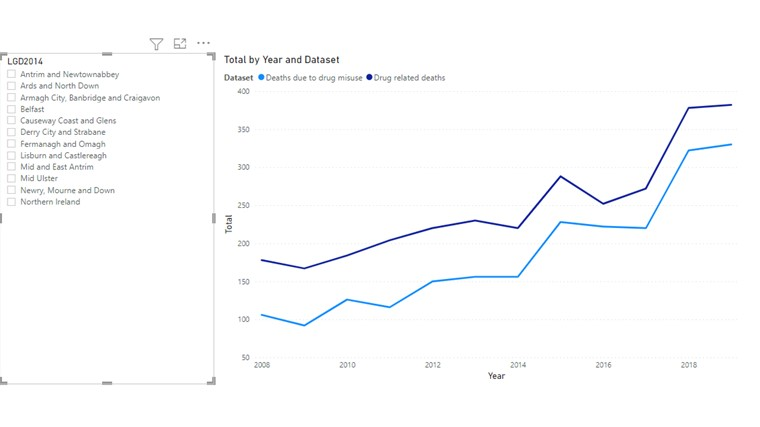
\includegraphics{bi8.jpg}
\caption{Filtering data by local government district (LGD).}
\end{figure}

\hypertarget{the-format-area}{%
\subsection{The Format Area}\label{the-format-area}}

We now have a line-chart that shows both deaths due to drug misuse and drug related deaths but if we control click multiple local government districts it sums them together. We can change this behaviour by formatting the slicer visual.

Click the \textbf{slicer visual} then click on the \textbf{Format area selector} (the icon that looks like a paint roller). We will be presented with a list of different attributes that we can change. We can change the title, the background, the border and we can add shadows. The important attribute we want to change however is \textbf{Selection controls}. Click the \textbf{drop-down arrow} beside \textbf{Selection controls} and toggle \textbf{single select} on. The result should be something that looks like this:

\begin{figure}
\centering
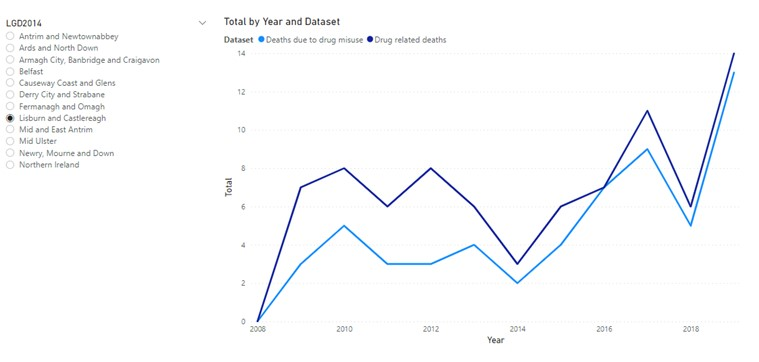
\includegraphics{bi9.jpg}
\caption{Filtering data by local government district (LGD) and selecting different regions.}
\end{figure}

This presentation style has positives and negatives. It's useful if we know we have lots of visitors who only want to know about their local government district but it's not very good for comparing different districts. We're going to use what we have done so far to build a new visual that allows users to directly compare their local government district to another.

Our line-chart visual will use LGD2014 as its legend. Our slicer will have to enable multiple selection. We may also want to include additional slicers to filter the visual by year and by the data set we would like to compare. We will also convert the visual type to a stacked bar chart. The final result should look like this:

\begin{figure}
\centering
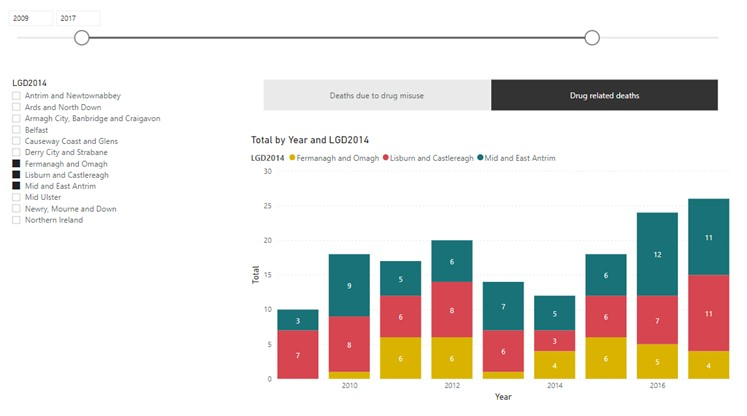
\includegraphics{bi10.jpg}
\caption{The Finished Product.}
\end{figure}

The new visual should allow us to check multiple boxes and add to the stacked bar chart. We should also be able to filter by year using the slider at the top and we should be able to select the data set we're interested in using the buttons above the visual.

\hypertarget{adding-new-pages}{%
\chapter{Adding New Pages}\label{adding-new-pages}}

\begin{center}\rule{0.5\linewidth}{0.5pt}\end{center}

\hypertarget{adding-a-new-page}{%
\section{Adding a New Page}\label{adding-a-new-page}}

We can add a new page to our report by clicking the plus sign \textbf{+} next to the \textbf{Page 1 tab} at the bottom of the canvas. It makes sense however to duplicate our existing page since we can re-use some of our existing work. \textbf{Right click} on the \textbf{Page 1 tab} and select \textbf{Duplicate Page}.

Select the \textbf{line-chart visual} and change the \textbf{legend} in the \textbf{Fields Area} from \textbf{Dataset} to \textbf{LGD2014} by clicking on the \textbf{X} to the right of \textbf{Dataset} and dragging in \textbf{LGD2014} from the \textbf{Fields Pane}. Now click on the \textbf{stacked column char}t icon in the \textbf{Visualizations Pane} to convert the visual. Some conversions work better than others, it's always worth checking that the visual is showing the same data before and after conversion. A conversion from a stacked bar chart to a card visual or KPI visual may not be the best choice for instance.

We will need to edit the location filter (the slicer) to allow for multiple selections. Click on the \textbf{slicer visual} and go to the \textbf{Format Area}. Under \textbf{Selection Controls} toggle \textbf{Single Select} to \textbf{off} and ensure that \textbf{Multi-select with CTRL} is toggled to the \textbf{on} position and \textbf{Show ``Select All'' Option} is toggled to the \textbf{off} position. We can now select multiple local government districts and they should stack on top of one another in the stacked bar chart visual. We will need two new slicer visuals.

Click on the canvas to ensure no visuals are selected. Select the \textbf{Slicer Visual} in the visualizations pane. Drag the \textbf{Year field} into the \textbf{Field box}. The slicer should automatically detect numeric data and generate a slider that takes values in the range 2008 to 2019.

We need one more slicer. Again ensure no visuals are currently selected and select the \textbf{Slicer Visual}. Drag the \textbf{Dataset} field into the slicer's field. A checkbox will be generated. We would prefer buttons this time, so go to the \textbf{Format Area} and select the \textbf{General} option. Scroll down until you see \textbf{Orientation}. Click on the drop down menu and select \textbf{Horizontal}. Under \textbf{Selection Controls} you might want to toggle \textbf{Single select} to \textbf{on}.

Finally, we can add some data labels to our visual. Select the line-chart visual by clicking on it. In the Format Area scroll down until you see \textbf{Data Labels} and toggle them \textbf{on}.

\hypertarget{navigation}{%
\chapter{Navigation}\label{navigation}}

\begin{center}\rule{0.5\linewidth}{0.5pt}\end{center}

\hypertarget{navigation-1}{%
\section{Navigation}\label{navigation-1}}

There are a number of methods to provide users with a means to navigate their way through a dashboard.

\hypertarget{arrows}{%
\subsection{Arrows}\label{arrows}}

Up to this point we have mostly made use of the Home ribbon but there are other important ribbons when designing reports. The \textbf{Insert ribbon} for instance allows us to insert elements into our report that aren't necessarily data visualizations. We can insert text boxes, buttons, shapes and images. These are all useful for providing additional information on visualizations, explaining data or navigation. We're going to create navigation buttons.

Add two new pages to your report using the plus icon next to the page tabs at the bottom of the canvas. Click onto the first of those pages. Then navigate to the \textbf{Insert ribbon} and click on \textbf{Buttons} then on the \textbf{right arrow}.

\begin{figure}
\centering
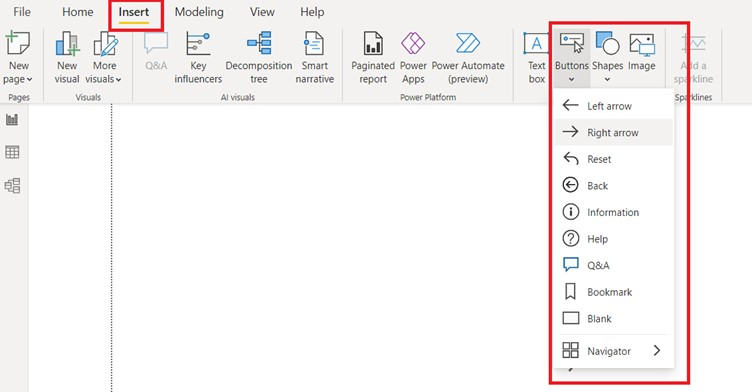
\includegraphics{bi11.jpg}
\caption{Inserting arrows.}
\end{figure}

Repeat this process on the second page but this time select the \textbf{Left arrow}. If the Left arrow is selected you will see the visualisations pane disappear and the entire pane will be taken up by the format pane. Scroll down until you find \textbf{Action}. Toggle \textbf{Action} to \textbf{on} and select \textbf{Page navigation} in the \textbf{Type menu} and \textbf{Page 1} (or whatever page you want this arrow to direct to) in the \textbf{Destination menu}.

\begin{figure}
\centering
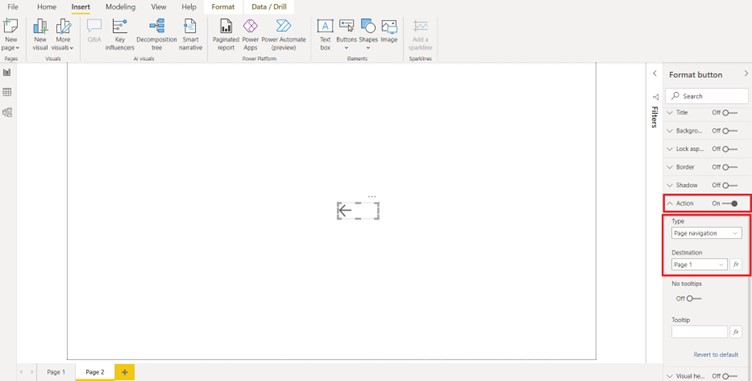
\includegraphics{bi12.jpg}
\caption{Left Arrow Navigation.}
\end{figure}

If you \textbf{CTRL+Click} on the \textbf{Left arrow} it should now take you to \textbf{Page 1}. When your Power BI Report is published users won't need to CTRL+Click it will just happen with a click. We can repeat these steps for the Right Arrow on Page 1 to cycle between the pages.

\hypertarget{buttons}{%
\subsection{Buttons}\label{buttons}}

Another useful element that we can insert is the \textbf{Button}. The Button can serve just about any purpose. It can be filled with color and used as a banner or a footer; it can be used as a navigation tool thanks to the actions we just used; and it can be used as a display behind a visual.

Create a new page. Find \textbf{Buttons} on the \textbf{Insert ribbon}. Click it and select \textbf{Blank}. An outlined box should appear. You can click the edges of this to resize it. Try to take up the whole width available and just less than 20\% of the height. It doesn't need to be exact, just resize to whatever looks natural as a header for a title.
Click on the resized button when you're finished. In the \textbf{Format Button pane} toggle \textbf{Outline} to \textbf{off} and toggle \textbf{Icon} to \textbf{off}. Toggle \textbf{Fill} to \textbf{on} and expand the fill menu and select a new color for your header. Change the transparency settings if you like. Next, find the \textbf{Text toggle} and toggle it \textbf{on} if it isn't already. Open the \textbf{Text menu} by clicking the drop-down arrow. In the text box type a title for your new page. You can change the font color and text size and the font below the text entry box.

Add another button but this time resize it to whatever size you think appropriate for a navigation button. Repeat the steps above to add colour and text to the button. Then you can use the action menu, like we did when we created the left and right arrows, to give the button navigation properties.

With any luck you should be able to replicate the kind of user interface you see in a \textbf{single page web app} or a \textbf{mobile app}.

\begin{figure}
\centering
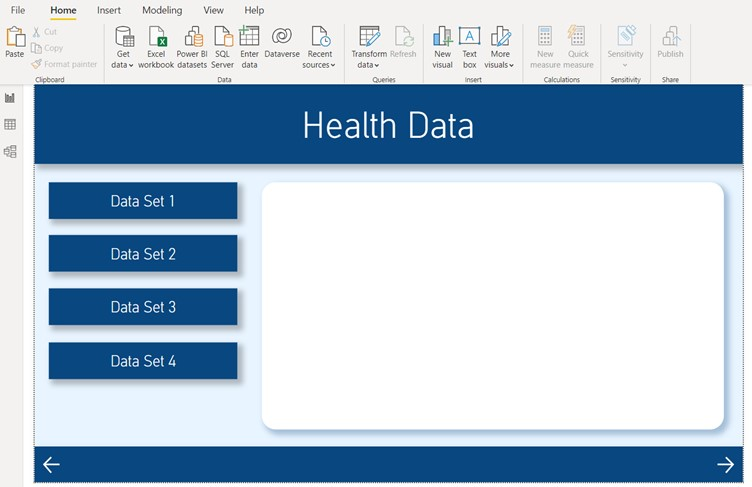
\includegraphics{bi13.jpg}
\caption{Buttons used to create links between pages.}
\end{figure}

\hypertarget{indexing}{%
\chapter{Indexing}\label{indexing}}

\begin{center}\rule{0.5\linewidth}{0.5pt}\end{center}

\hypertarget{indexing-1}{%
\section{Indexing}\label{indexing-1}}

This example will show you how to create a bar chart visual of sales by month. This sounds simple but often when trying to visualise data categorised by month the bars for each month are sorted by alphabetical order rather than the order in which the months occur.

Start a new project and click \textbf{Enter Data}.

Enter the months of the year in the available column and change the column title to ``Month''.

Press the \textbf{+} Icon at the top right to create a new column, title it ``Sales'' and enter some dummy sales data.

\begin{figure}
\centering
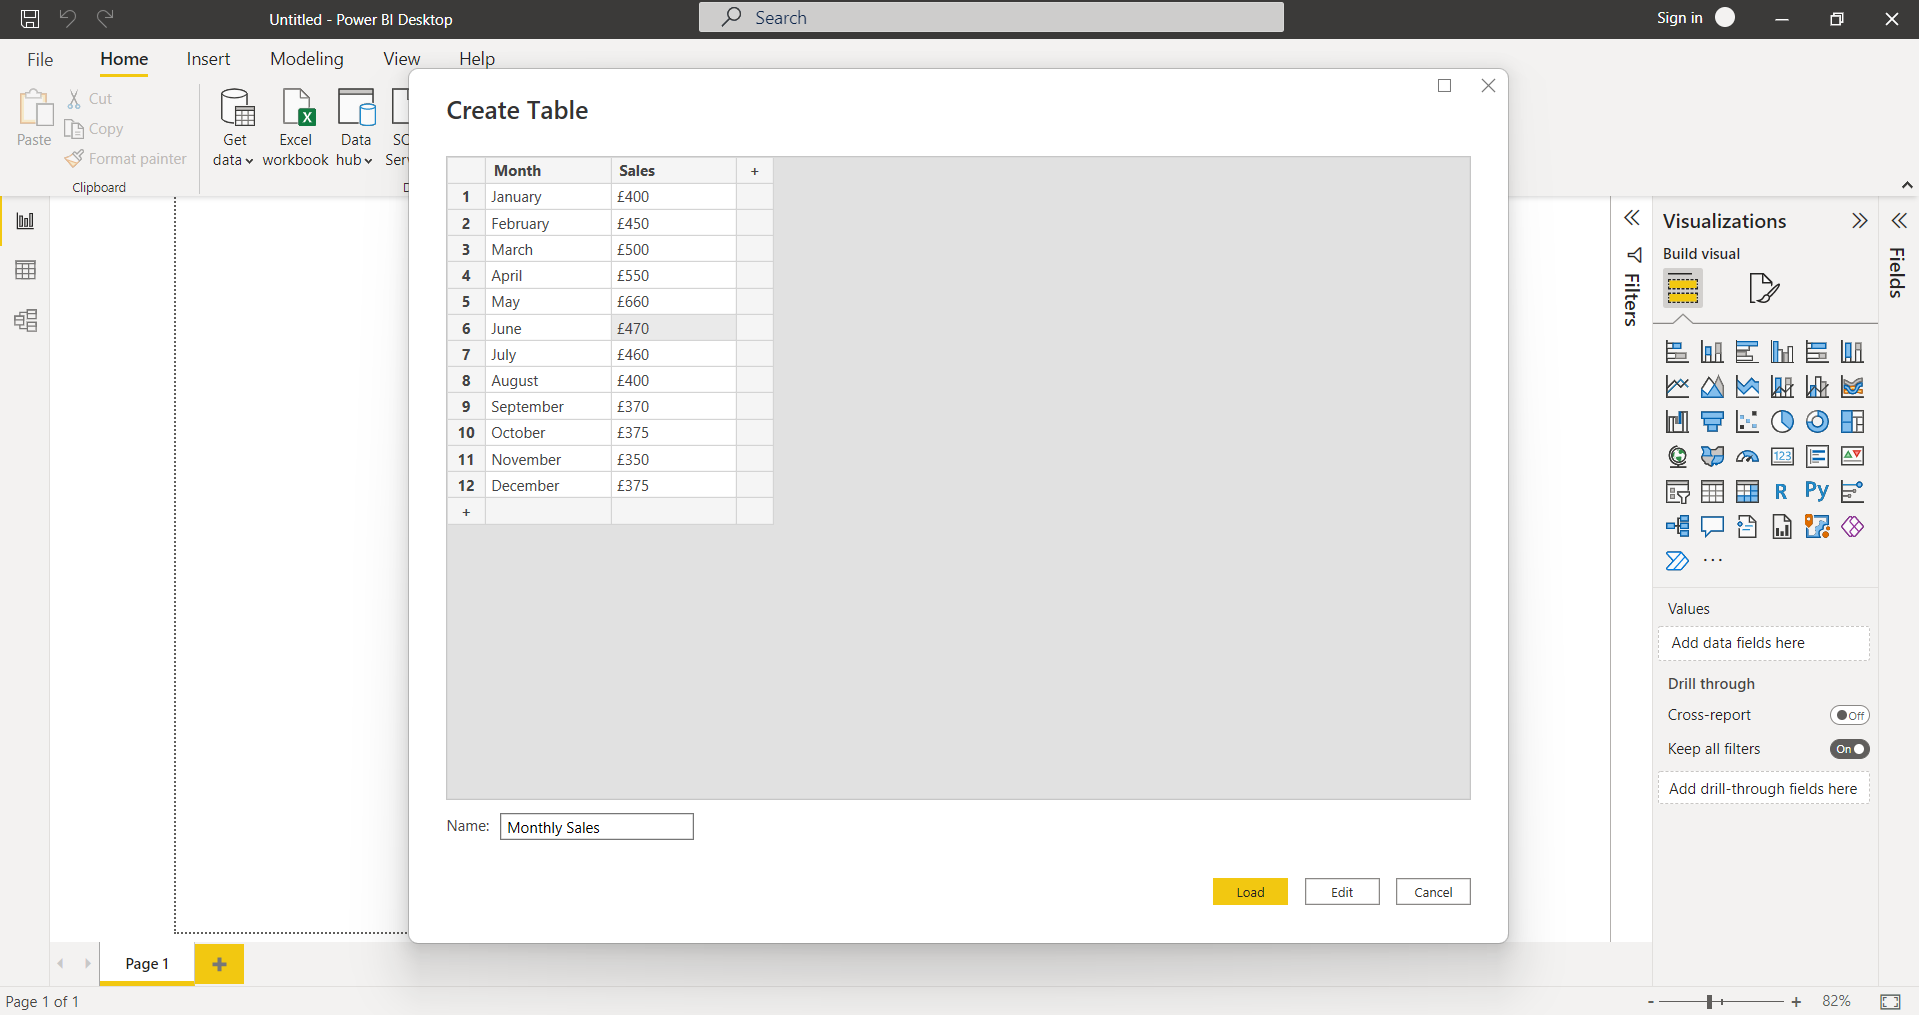
\includegraphics{bi14.png}
\caption{Entering data}
\end{figure}

Load the data.

Create a bar chart visualisation with ``Month'' in the X-axis field and ``Sales'' in the Y-axis field.

Once the visualisation has been created click the \textbf{\ldots{}} icon for more options and sort the axis by month. The x-axis will be sorted by month but it will be sorted alphabetically.

To rectify this we need to create an \textbf{index}.

Click on \textbf{Transform Data} and navigate to ``Monthly Sales''. In \textbf{Applied Steps} pane on the right hand side there will be a step called \textbf{Source} with a cog icon to the right of it. Click on the cog. This will open up the editor you used to input the data. Create a new column by clicking the \textbf{+} icon. Call this new column ``Index'' and write the number 1 in the first empty row. Write the number 2 in the next row and the number 3 in the next. Continue until each Month has a corresponding numerical index.

\begin{figure}
\centering
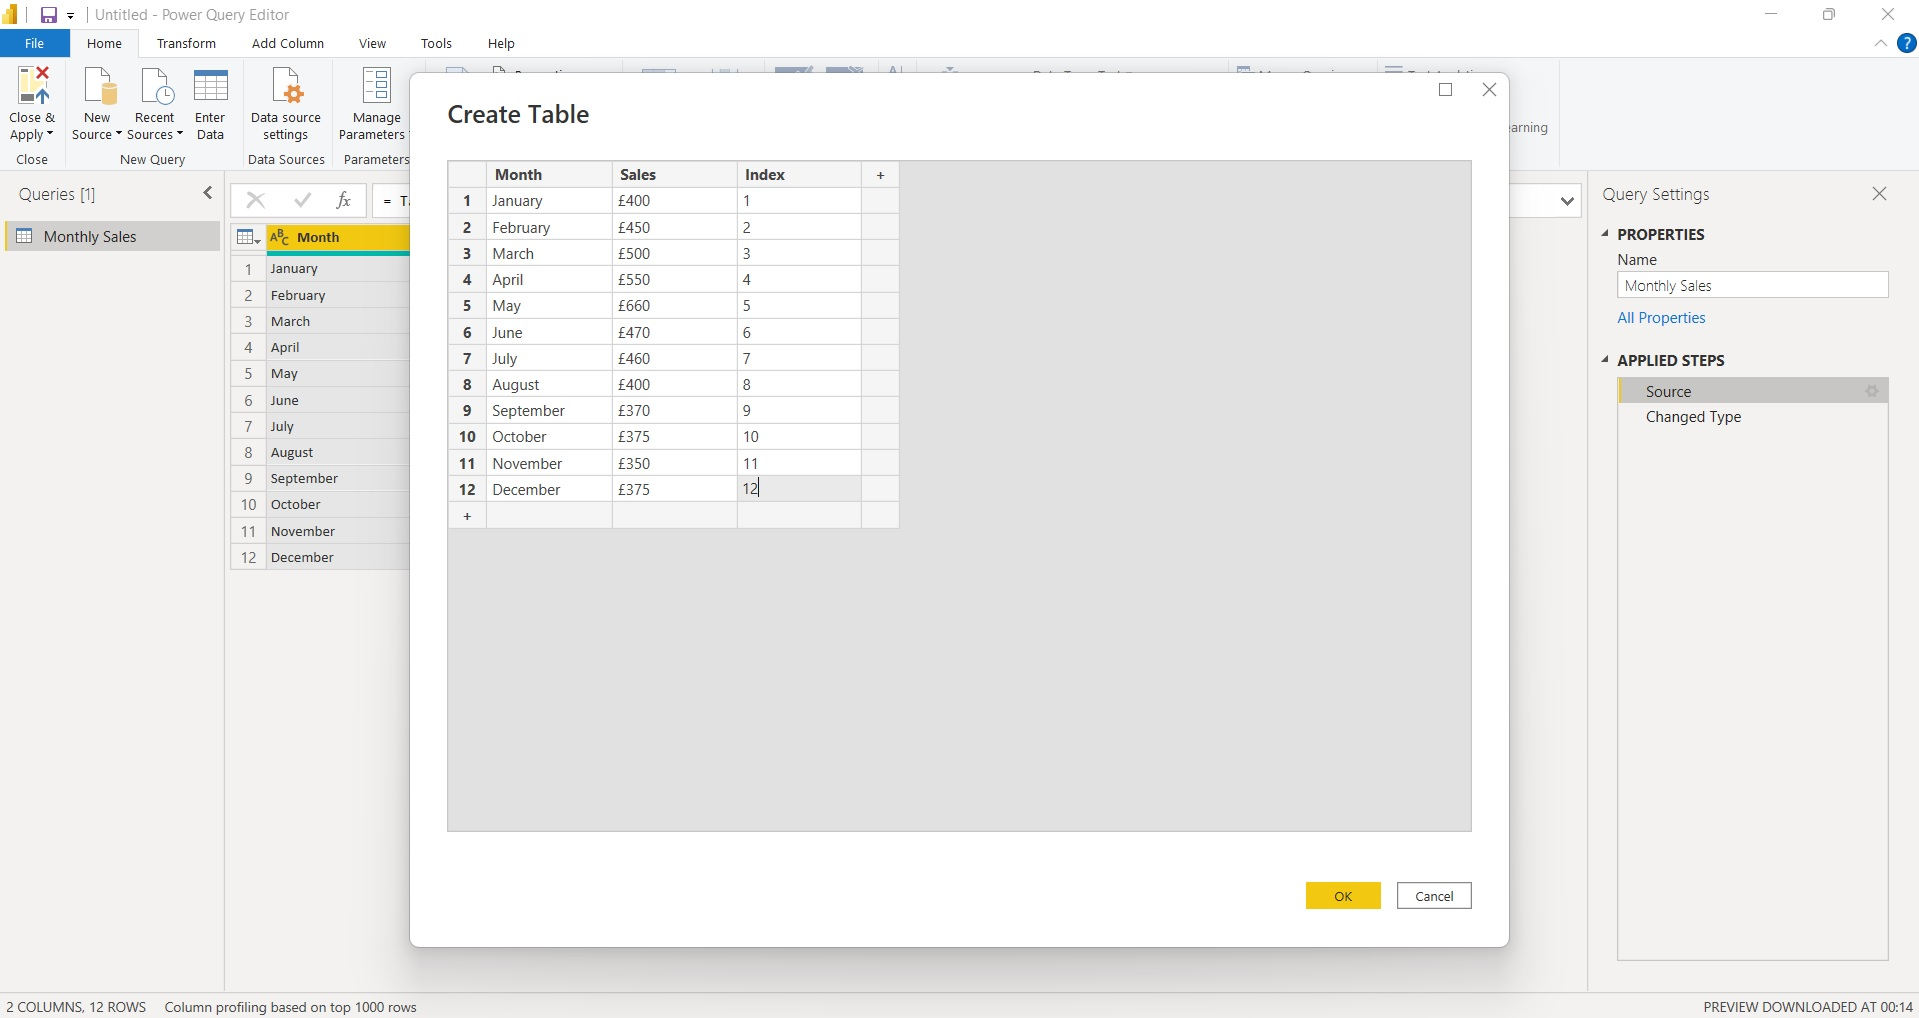
\includegraphics{bi15.jpg}
\caption{Creating an index}
\end{figure}

When finished, click \textbf{OK} then \textbf{Close \& Apply}.

Go to the data view, click on the ``Month'' column and find the \textbf{Sort by column} option in the \textbf{column tools} ribbon and select ``Index''.

\begin{figure}
\centering
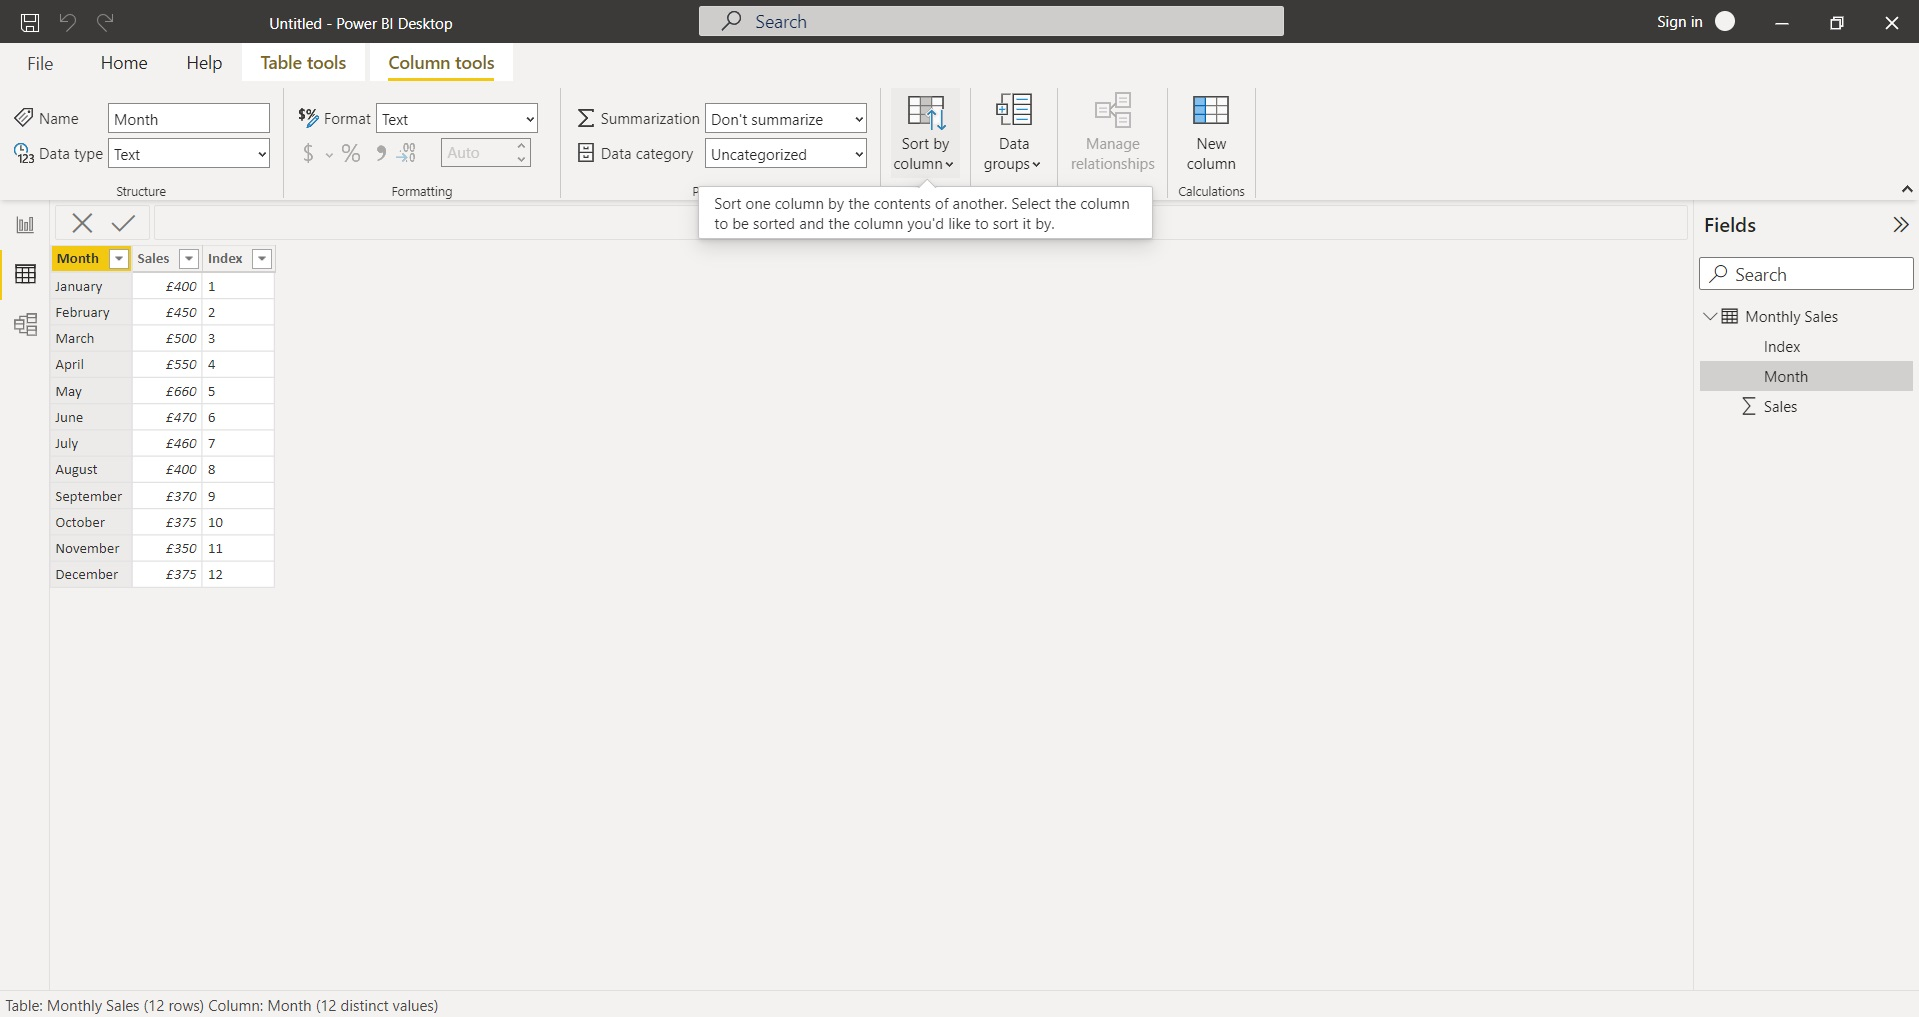
\includegraphics{bi16.jpg}
\caption{Sorting by column}
\end{figure}

Return to the visualisation and the months should now be sorted in the correct order.

\hypertarget{relationships}{%
\chapter{Relationships}\label{relationships}}

\begin{center}\rule{0.5\linewidth}{0.5pt}\end{center}

\hypertarget{publishing}{%
\chapter{Publishing}\label{publishing}}

\begin{center}\rule{0.5\linewidth}{0.5pt}\end{center}

\hypertarget{sharing}{%
\chapter{Sharing}\label{sharing}}

\begin{center}\rule{0.5\linewidth}{0.5pt}\end{center}

\hypertarget{additional-resources}{%
\chapter{Additional Resources}\label{additional-resources}}

\begin{center}\rule{0.5\linewidth}{0.5pt}\end{center}

\hypertarget{additional-resources-1}{%
\section{Additional Resources}\label{additional-resources-1}}

This content has been designed to provide a tour of the main features of Power BI reports. It has skipped a lot of detail to try and give a broad overview of what is possible with Power BI and provide the basic skills needed to start experimenting with the software package.

\hypertarget{power-bi-documentation}{%
\subsection{Power BI Documentation}\label{power-bi-documentation}}

The \href{https://docs.microsoft.com/en-us/power-bi/fundamentals/}{Power BI Documentation} should provide a more in depth look at the fundamentals. Microsoft Learn has a number of \href{https://docs.microsoft.com/en-us/learn/modules/get-started-with-power-bi/}{modules} dedicated to Power BI which are mostly related to Data Analysis learning pathways. Completing these modules will be useful for consolidating the fundamentals and learning more about Power BI in greater detail.

\hypertarget{dax}{%
\subsection{DAX}\label{dax}}

If you're really interested then it might be worth reading into \href{https://docs.microsoft.com/en-us/dax/}{Data Analysis Expressions (DAX)} which is a library of functions that can be used to build formulas and expressions in Power BI, Analysis Services, and Power Pivot in Excel data models. This is especially useful in Power Query Editor.

  \bibliography{book.bib,packages.bib}

\end{document}
